%%%%%%%%%%%%%%%%%%%%%%%%%%%%%%%%%%%%%%%%%
% Beamer Presentation
% LaTeX Template
% Version 1.0 (10/11/12)
%
% This template has been downloaded from:
% http://www.LaTeXTemplates.com
%
% License:
% CC BY-NC-SA 3.0 (http://creativecommons.org/licenses/by-nc-sa/3.0/)
%
%%%%%%%%%%%%%%%%%%%%%%%%%%%%%%%%%%%%%%%%%

%----------------------------------------------------------------------------------------
%	PACKAGES AND THEMES
%----------------------------------------------------------------------------------------

\documentclass{beamer}

\usepackage{booktabs}% http://ctan.org/pkg/booktabs
\newcommand{\tabitem}{~~\llap{\textbullet}~~}
%\usepackage{enumitem}
\usepackage{adjustbox}
\usepackage{anyfontsize}
%\usepackage{fontspec}

\usepackage{tikz}
%\setmainfont{CMU Serif}

\mode<presentation> {

\usepackage{changepage}
%\usetheme{Warsaw}
\usetheme{Madrid}
%\setbeamertemplate{footline} % To remove the footer line in all slides uncomment this line
%\setbeamertemplate{footline}[page number] % To replace the footer line in all slides with a simple slide count uncomment this line

\setbeamertemplate{navigation symbols}{} % To remove the navigation symbols from the bottom of all slides uncomment this line
}

\usepackage{graphicx} % Allows including images
\usepackage{booktabs} % Allows the use of \toprule, \midrule and \bottomrule in tables
\usepackage[keys]{cryptocode}

%----------------------------------------------------------------------------------------
%	TITLE PAGE
%----------------------------------------------------------------------------------------

\title[mpOTR]{Multi party Off-the-Record messaging protocol} % The short title appears at the bottom of every slide, the full title is only on the title page

\author[Andrikopoulos, Kolotouros]{~Andrikopoulos Konstantinos\inst{1} \and ~Kolotouros Dimitrios\inst{2}} % Your name
\institute[NTUA] % Your institution as it will appear on the bottom of every slide, may be shorthand to save space
{
  \inst{1}%
  National Technical University of Athens 
\includegraphics[scale=0.1]{Figures/Pyrforos.png} \\ % Your institution for the title page
  \textit{gkonstandinos@gmail.com} % Your email address
  \and
  \inst{2}%
  National Technical University of Athens 
\includegraphics[scale=0.1]{Figures/Pyrforos.png} \\ % Your institution for the title page
  \textit{dim.kolotouros@gmail.com} % Your email address
\medskip
}
\date{Febuary 22, 2016} % Date, can be changed to a custom date


\begin{document}

\begin{frame}
\titlepage % Print the title page as the first slide
\end{frame}

\begin{frame}
\frametitle{Overview} % Table of contents slide, comment this block out to remove it
\tableofcontents % Throughout your presentation, if you choose to use \section{} and \subsection{} commands, these will automatically be printed on this slide as an overview of your presentation
\end{frame}

%----------------------------------------------------------------------------------------
%	PRESENTATION SLIDES
%----------------------------------------------------------------------------------------

\chapter{Introduction}

\label{chapter:introduction}

\newcommand{\dhname}{Diffie--Hellman }
\newcommand{\tdhname}{Triple Diffie--Hellman }


%--------------------------------------------

\section{Motivation}
Not much time has passed since Edward Snowden revealed the plans that a certain intelligence agency has for the internet. While the world had always been suspecting that the various 3-letter agencies had the capability of controlling the network at a large scale, everybody was shocked with the confirmation of those suspicions.

In a world where the need for easy instant communication must overcome the threat of constant surveillance, end-to-end encryption has become a necessity. It's not a coincidence that digital privacy has come into focus during the last years. One after another companies advertise the utilization of encryption in their products. Apparently, Instant Messaging is the most favorable means of communication when it comes to end-to-end encryption.

One of the oldest and commonly used protocols that provides privacy in Instant Messaging is the Off-The-Record (OTR). OTR was initially introduced in a paper named "Off-the-Record Communication, or, Why Not To Use PGP" in 2004 \cite{otr} and later improved in \cite{otr_improvedauth}. It was named after the homonymous method of journal sourcing. The primary motivation behind OTR was to provide deniable authentication for the conversation participants while keeping conversations confidential, as in real-life private conversations. The protocol is implemented as a C library and a Pidgin plugin, a user study of which can be found in \cite{otr_userstudy}.

Unfortunately, OTR does only apply in a two-party setting, where only two participants are exchanging messages. However, multi-party chat rooms are also very prominent in everyday communications. A protocol providing the same privacy properties as OTR in a multi-party setting was theoritically described in the "Multi-party Off-the-Record Messaging" paper by I. Goldberg et al. in 2009 \cite{mpotr}. This protocol is called multi-party OTR (mpOTR). Although it's been around since 2009, no actual implementation of mpOTR existed until now.

\section{Our Contributions}
The existing theoretical introduction of mpOTR protocol in \cite{mpotr} treats the underlying subrotocols as black boxes and does not describe them in detail. More specifically, two underlying subprotocols are left unspecified, namely the deniable Authenticated Key Exchange (denAKE) and the Group Key Agreement (GKA). These sub-protocols play a key role in setting up the parameters needed for authentication and encryption.

We propose a full construction for the mpOTR Protocol. We specify every underlying sub-protocol. We also specify all the primitive algorithms used for several cryptographic functions, such as hashing, signing and encrypting. Finally, we propose a detailed low-level description of the protocol, including message structures, encoding, etc.

In addition, we provide the first implementation of mpOTR. Our implementation is a production-grade extension of the existing OTR library accompanied by a pidgin plugin, all writen in C. Both are open source projects, available in our github repositories\footnote{https://github.com/Mandragorian/libotr}\footnote{https://github.com/Mandragorian/pidgin\_otr}. We engineered our implementation in such a way that its security is easily reviewable, and, at the same time, facilitates the free software development model, where contributions in the source code are made from several independent authors.

\section{Outline}
In Chapter \ref{chapter:theoretic_background} we introduce some basic theoretic background. All the concepts, cryptographic primitives, and ideas presented there are essential building blocks of the mpOTR Protocol construction proposed in this thesis.

In Chapter \ref{chapter:threat_model} we specify the threat model of the mpOTR Protocol. We describe the different types of adversaries along with their goals. Then, we describe the goals of the mpOTR Protocol to achieve security against each type of adversary.

In Chapter \ref{chapter:protocol} we present our mpOTR Protocol construction. First, we specify the desirable privacy properties of mpOTR conversations and the underlying network setting. Then, we present a high-level overview of the protocol followed by a detailed description of every building block. Afterwards, we specify several technical details. Finally, we specify the exact structure of the messages exchanged in mpOTR.

In Chapter \ref{chapter:implementation} we present our actual implementation of mpOTR. We introduce  several design challenges and the relevant decisions. Then we present the design model of the mpOTR library. Finally, we specify the Application Programming Interface that our implementation offers to the IM applications in order to utilize mpOTR in group conversations.

In Chapter \ref{chapter:plugin} we present our modifications of the OTR pidgin plugin. We introduce the Graphical User interface and the workflow of a private group conversation.

In Chapter \ref{chapter:related_work} we present other protocols that utilize end-to-end encrpytion in multi-party context.

In Chapter \ref{chapter:future_work} we present several problems regarding specific parts of our mpOTR construction. While our construction is fully functional and secure, solving these problems would enhance the protocol’s privacy and/or usabilty. We fully describe each of them and suggest possible solutions.
\section{Offer}
\begin{frame}
\Huge{\centerline{Offer}}
\end{frame}

\begin{frame}
  This subprotocol does two things simultaneously.
  \vfill
  First the initiator makes an offer to other participants to start a session.
  \vfill
  Secondly, it generates a unique session ID for this run of the protocol.
\end{frame}

\begin{frame}
  The problem: Messages from one chatroom should not be valid in another chatroom.
  \vfill
  The solution: Create a (with high probability) unique session id. This way any signatures will not be valid in other chatrooms.

\end{frame}

\begin{frame}
  To achieve that, each user $A$ generates a random number $c_A$, called the contribution.
  \vfill
  She then transmits her contribution to everyone else in the chatroom.
  \vfill
  She calculates the session id when she has received the contributions from all other users.
  \[
      sess_{id} = H(c_A || c_B || \dots || c_Z)
  \]
  \vfill
  $sess_{id}$ is not authenticated, but we fix that later.
\end{frame}

\section{Deniable Signature Key Exchange}

\begin{frame}
\Huge{\centerline{DSKE}}
\end{frame}

\begin{frame}
  \frametitle{DSKE}
  This subprotocol constructs an association table between participants and the keys they will use for message signing.\\[0.3cm]

  Any information transmitted during this protocol is:

  \begin{itemize}
    \item Authenticated
    \item Deniable
  \end{itemize}

  This would be the image of the chat room just after the DSKE is finished:
  \begin{figure}
    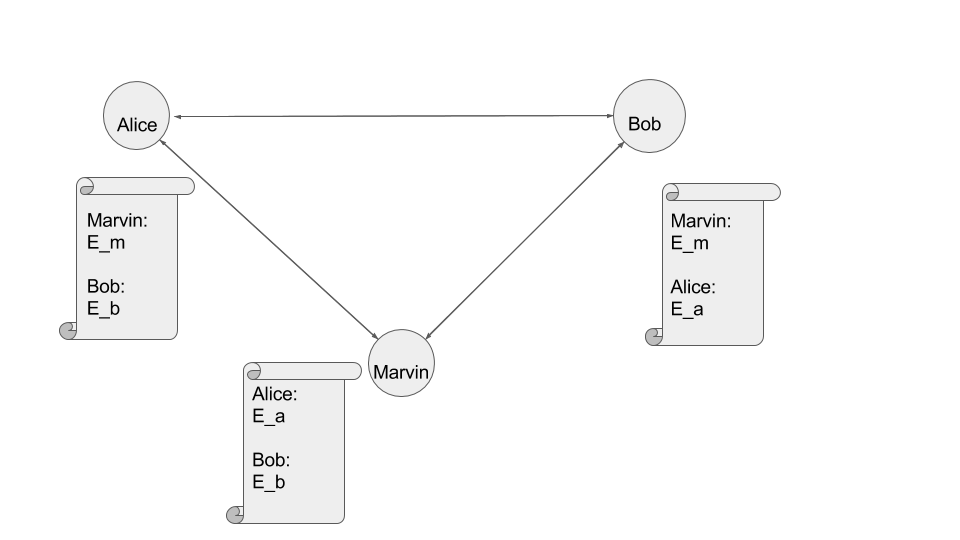
\includegraphics[scale=0.2]{Figures/denAKE.png}
  \end{figure}
\end{frame}

\begin{frame}
  To achieve that, DSKE assumes the existance of a subprotocol called \emph{Deniable Authenticated Key Exchange} (denAKE).\\[0.3cm]

  The denAKE protocol creates an {\bf authenticated} and {\bf deniable} shared secret between two participants. Using that shared secret the two participants send each other the public key they will be using. This is done for every pair of participants.\\[0.3cm]

  \begin{minipage}{.47\textwidth}
    In our implementation denAKE is implemented using the triple diffie hellman where the shared secret is:

    \[
      s = g^{Xy} || g^{xY} || g^{xy}
    \]

  \end{minipage}
  \begin{minipage}{.47\textwidth}
     \begin{figure}
      \scalebox{0.5}{ \begin{tikzpicture}

  \def \dist {5cm}
  \def \longrad {1cm}
  \def \ephemrad {0.8cm}
  \def \sqrttwo {1.4142}

  \node[draw, circle, minimum size=\longrad] at (0,\dist) {$X$};
  \node[draw, circle, minimum size=\ephemrad] at (0,0) {$x$};
  \node[draw, circle, minimum size=\longrad] at (\dist,\dist) {$Y$};
  \node[draw, circle, minimum size=\ephemrad] at (\dist,0) {$y$};

  \draw[<->, >=latex] ({0 + (\sqrttwo * \longrad / 4)} ,{\dist  - (\sqrttwo * \longrad / 4)})
  -- ({\dist - (\sqrttwo * \ephemrad /4)},{0 + (\sqrttwo * \ephemrad / 4)});

  \draw[<->, >=latex] ({\dist - (\sqrttwo * \longrad / 4)} ,{\dist  - (\sqrttwo * \longrad / 4)})
  -- ({0 + (\sqrttwo * \ephemrad /4)},{0 + (\sqrttwo * \ephemrad / 4)});

  \draw[<->, >=latex] ({0 + \ephemrad/2}, 0) -- ({\dist - \ephemrad/2}, 0);

\end{tikzpicture}
}
    \end{figure}
  \end{minipage}
\end{frame}

\begin{frame}
  \begin{figure}
    \scalebox{0.39}{\fbox{%
  \pseudocode{%
    \textbf{Alice} \< \< \textbf{Bob} \\[][\hline]
    \text{ Choose a random number $x \in Z_p^*$ }\< \< \\
    \< \sendmessageright*{Send \ \left(g^x,g^X\right)} \< \\
    \< \< \text{ Choose a random number $y \in Z_p^*$ } \\
    \< \< s = g^{xy} || g^{Xy} || g^{Yx} \\
    \< \< k_1 = KDF_1(s) \\
    \< \< k_2=KDF_2(s) \\
    \< \sendmessageleft*{Send \ \left(g^y,g^Y\right)} \< \\
    s = g^{xy} || g^{Xy} || g^{Yx} \< \< \\
    k_1 = KDF_1(s) \< \< \\
    k_2 = KDF_2(s) \< \< \\
    \< \sendmessageright*{ Send \\ c = AES_{k_1}("confirm") \\ MAC_{k_2}(c)\ } \< \\
    \< \< \text{Verify mac} \\
    \< \< m = AES^{-1}_{k_1}(c) \\
    \< \< \text{Verify m = "confirm"} \\
    \< \sendmessageleft*{ Send \\ c = AES_{k_1}("confirm") \\ MAC_{k_2}(c)\ } \< \\
    \text{Verify mac} \< \< \\
    m = AES^{-1}_{k_1}(c) \< \< \\
    \text{Verify m = "confirm"} \\
    \< \sendmessageright*{Send \\ c = AES_{k_1}(\pk_a) \\ MAC_{k_2}(c) } \< \\
    \< \< \text{Verify mac} \\
    \< \< \text{Add $\pk_a$ to association table} \\
    \< \sendmessageleft*{Send \\ c = AES_{k_1}(\pk_b) \\ MAC_{k_2}(c) } \< \\
    \text{Verify mac} \< \<  \\
    \text{Add $\pk_b$ to association table} \< \< \\
  }
}

}
  \end{figure}
\end{frame}

\section{Shutdown}

\begin{frame}
\Huge{\centerline{Shutdown}}
\end{frame}

\begin{frame}
After we the participants are done communicating the protocol must shut down.
\vfill
During this phase the participants will

  \begin{itemize}
    \item Determine that there are no more messages in-flight.
    \item Verify the consistency of their transcripts.
    \item Destroy the session and delete any ephemeral secrets.
  \end{itemize}
\end{frame}


\begin{frame}
To establish that there is a consensus over the set of the messages, each participant $X$ hashes his \emph{sent} list (ordered lexicographically), producing the hash $h_x$ and broadcasts the tuple $\langle "shutdown", h_x \rangle$.\\[0.5cm]


\includegraphics[scale=0.4]{Figures/sent_hash.png}
\end{frame}

\begin{frame}
After that he will patiently wait to receive the shutdown message from all  other participants.\\[0.5cm]

When he receives a shutdown message from user $Y$ he shall hash on his own $Y$'s \emph{received} list  and mark that he is no longer waiting messages from user $Y$.\\[0.5cm]


\includegraphics[scale=0.4]{Figures/received_hashes.png}
\end{frame}

\begin{frame}
After he has received the shutdown messages from all users he will hash his \emph{sent} hash with all the received hashes together, producing a digest $h$ of the whole chat, and broadcasts the tuple $\langle "digest", h \rangle$.\\[0.5cm]


\includegraphics[scale=0.4]{Figures/chat_digest.png}
\end{frame}

\begin{frame}
He will again wait to receive the digest messages from all other users and compare the received digests with the one he produced earlier in order to determine if a consensus is reached.\\[0.5cm]


\includegraphics[scale=0.4]{Figures/determine_consensus.png}
\end{frame}

\begin{frame}
After that he informs the other users that he does not intend to send any messages, and waits to receive such confirmations from the rest of the users.\\[0.5cm]


\includegraphics[scale=0.4]{Figures/no_listen_verify.png}\\[1cm]

And finally he broadcasts his signing key.
\end{frame}

\end{document}
